\documentclass{article}
\usepackage{ctex}
\usepackage{graphicx}
\usepackage{amsmath}
\usepackage{indentfirst}
\usepackage{titlesec}
\usepackage{setspace}
\usepackage{subfigure}
\usepackage{caption}
\usepackage{float}
\usepackage{booktabs}
\usepackage{geometry}
\usepackage{multirow}
\usepackage{hyperref}
\hypersetup{
	colorlinks=true,
	linkcolor=blue,
	filecolor=magenta,      
	urlcolor=cyan,
	pdftitle={Overleaf Example},
	pdfpagemode=FullScreen,
}
\geometry{left=1.2cm,right=1.2cm,top=2cm,bottom=2cm}
\title{\songti \zihao{2}\bfseries HW6第11题DLA与DBM模拟}
\titleformat*{\section}{\songti\zihao{4}\bfseries}
\titleformat*{\subsection}{\songti\zihao{5}\bfseries}
\renewcommand\thesection{\arabic{section}}
\author{王启骅 PB20020580}
\begin{document}
	\maketitle
	\section{题目}
模拟2维DLA以及介电击穿(DBM)图案并讨论
	
	\section{算法原理}
\subsection{DLA}
运用2维DLA模型,首先生成一个二维$ L\times L=1001\times1001 $的mesh网格,用1作为生长点,0作为未生长的点。在网格中心$ (\frac{L+1}{2},\frac{L+1}{2}) $放置结晶核设置为1。


通过模拟发现可以使用$ start=a\sqrt{n} $作为生成粒子的半径位置。n为已产生的粒子数。则在这里在半径为$ start=1.2\sqrt{n} $的圆上,通过生成$ [0,2\pi] $均匀分布的随机数生成在圆上均匀产生的粒子。设定在粒子游走到$ edge=2.4\sqrt{n} $的圆外时认为消失,进行下一次模拟。当edge达到mesh网格的边界处时,即$ 2.4\sqrt{n}>\frac{L-1}{2}-1 $时,直接设定$ edge=\frac{L-1}{2}-1,start=edge-\frac{L}{100} $。如果游走到周围有格点为1时,则将该粒子所在的格点设为1,认为生长,并进行下一次模拟。
\subsection{DBM}
根据DBM模型,设定同上的网格,在中心设置结晶核1。根据边界条件,在这里设定已生长的格点$ \phi_0=1 $,远处的格点$ \phi=0 $ 。每次选取$ edge=3\sqrt{t} $作为边界无穷远半径,同样对于达到格点边界的情况有$ edge=\frac{L-1}{2}-1 $ 。t为已经生长的次数


首先从以中心为心的边长2edge的正方形内筛选出周围存在1格点的0格点,即为接下来生长的候选边界格点。接下来求解这些格点的拉普拉色方程得到电势$ \phi_{i,j} $ 。再次利用Monte Carlo模拟的方法。用n个粒子在(i,j)为出发点进行随机游走,到达edge处记$ \phi=0 $,到达1格点处即为$ \phi=1 $。为了程序运行速度,设定n=100。
\begin{equation}
	\langle\phi_{i,j}\rangle=\frac{1}{n}\sum_{k=1}^{n}\Phi(s^{(k)})
\end{equation}


接下来计算格点扩散生长速率
\begin{equation}
	v_{i,j}=(t+1)|\phi_0-\phi_{i,j}|^{\eta}
\end{equation}
其中$ \eta $为生长速率参数。

环绕一周格点占据几率
\begin{equation}
	p_{i,j}=\frac{v_{i,j}}{\sum v_{i,j}}
\end{equation}


利用生成[0,1]均匀分布的随机数选择出生长的点。
	\section{结果}
	在模拟中,为了程序简洁明了,这里分别分开用两个程序进行模拟DLA和DBM模型,分别为$HW6\_11\_DLA.f90  $和$ HW6\_11\_DBM.f90 $。
	
	
将计算出的生长格点mesh导入到txt文件中,读入python画图,以下模拟了粒子生长从100个粒子到$ 10^5 $个粒子的情况


 \begin{figure}[!h]
	\centering
	\subfigure[100个粒子]{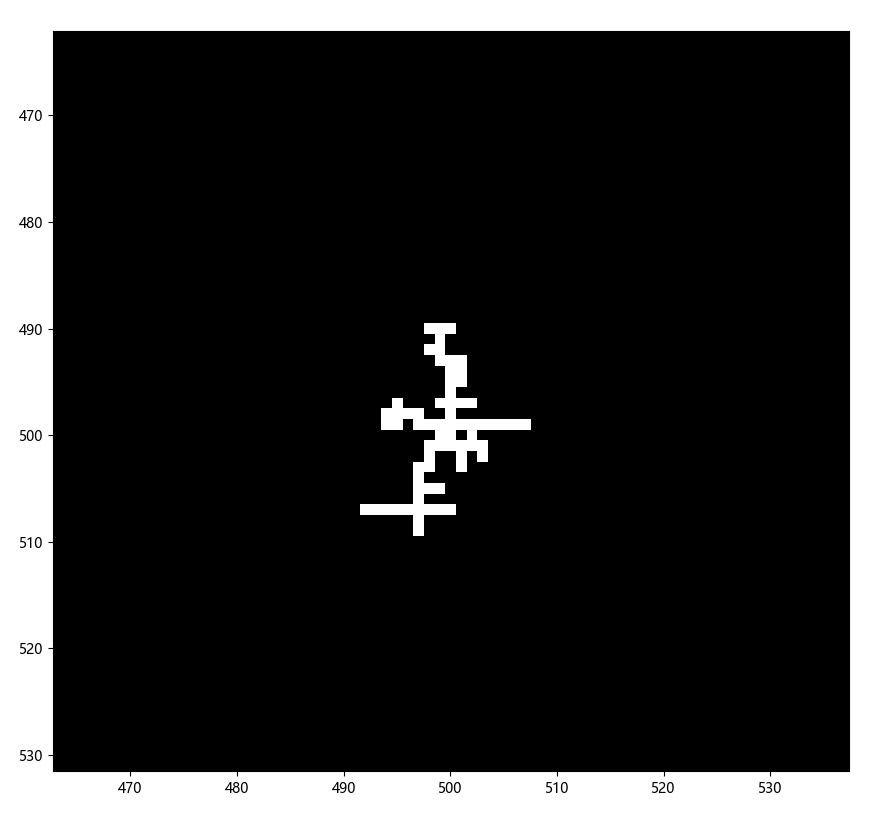
\includegraphics[scale=0.3]{DLA_2}}
	\subfigure[1000个粒子]{	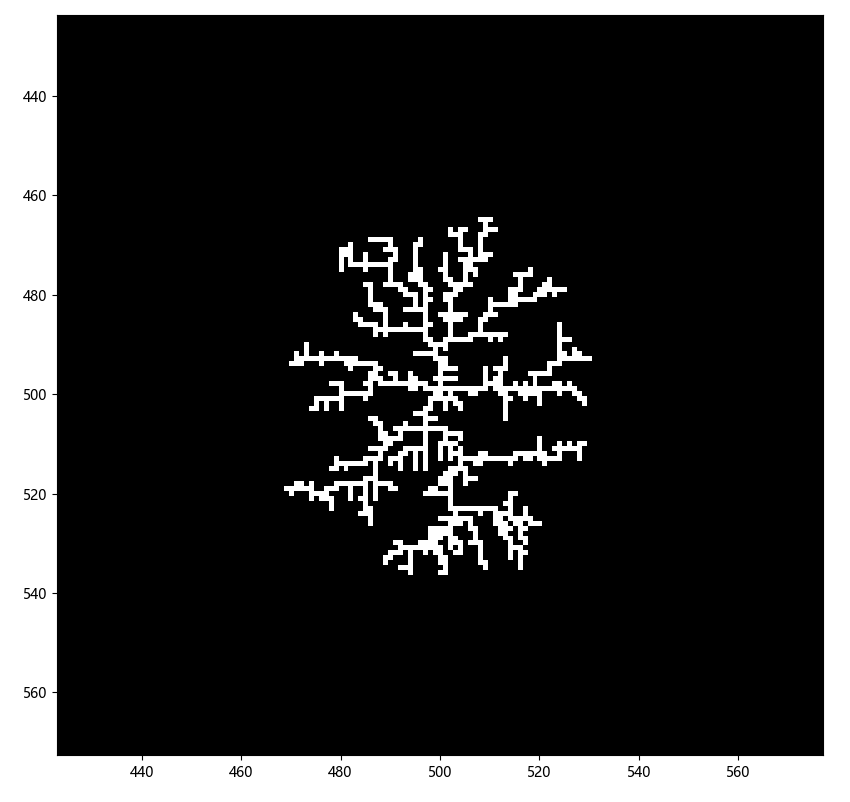
\includegraphics[scale=0.3]{DLA_3}}
	
	\subfigure[10000个粒子]{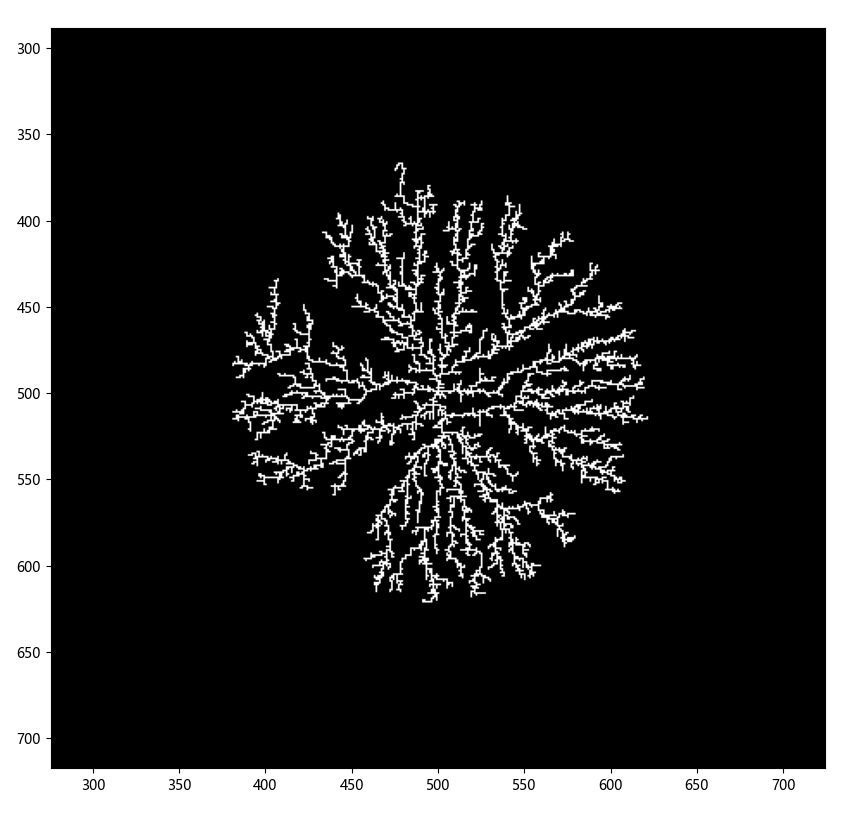
\includegraphics[scale=0.3]{DLA_4}}
	\subfigure[100000个粒子]{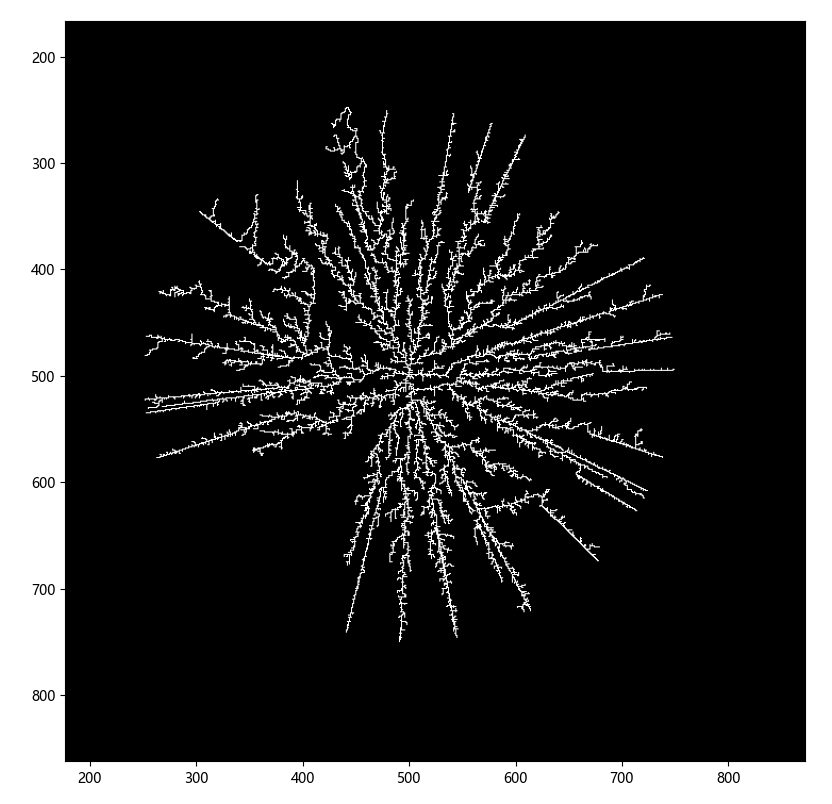
\includegraphics[scale=0.3]{DLA_5}}
	\captionsetup{font={small},labelfont=bf}
	\caption{\heiti\zihao{-5}DLA模拟}
	\label{fig:1}
\end{figure}


由图\ref{fig:1}分析可见,晶体生长的速率,即半径随粒子数的规律大致满足$ r\sim\sqrt{n} $的规律。并且晶体的结构从一开始较为不规则随着粒子数增加,逐渐更多的沿树枝增长,明显可见沿着尖端生长的趋势较强,整体趋于圆形向外扩散。


接下来分别用$ \eta=1,3,5,10 $,模拟了DBM生长,考虑到计算量较大,程序运算速度的问题,采用了$ 501\times501 $大小的网格进行模拟。图\ref{fig:2}模拟了$ \eta=3 $下生长次数t=100,300,700,1000,1500,2000下的生长图,由图可见DBM生长具有明显的方向性,沿着某一特定方向生长,并且有着较强的尖端生长趋势,到生长的末端由于逐渐靠近边界会逐渐扩散开。
 \begin{figure}[!h]
	\centering
	\subfigure[t=100]{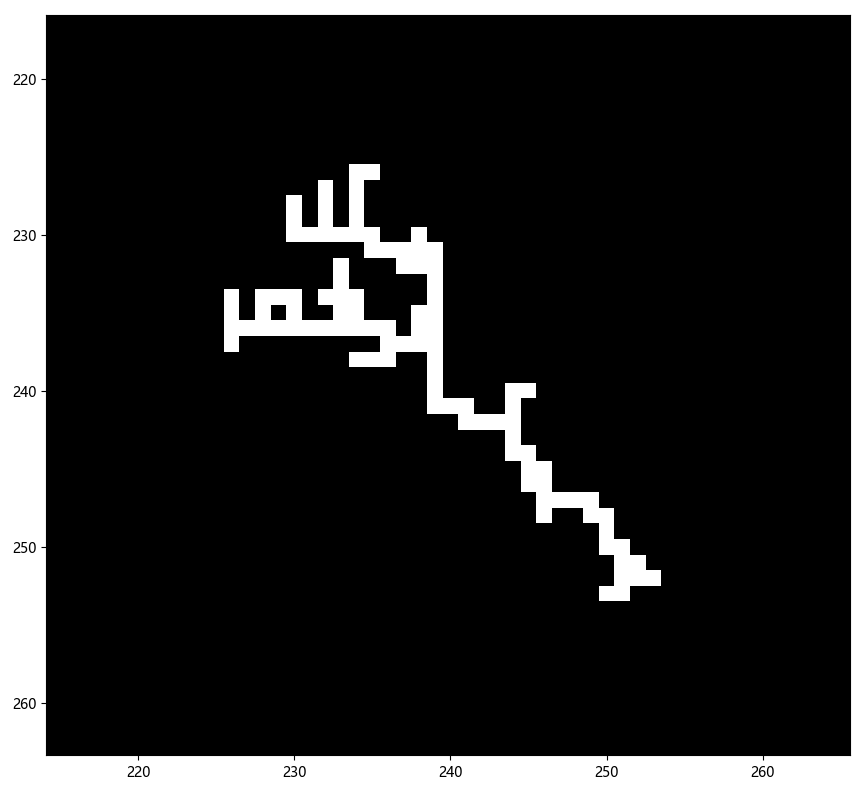
\includegraphics[scale=0.3]{DBM_3_100}}
	\subfigure[t=300]{	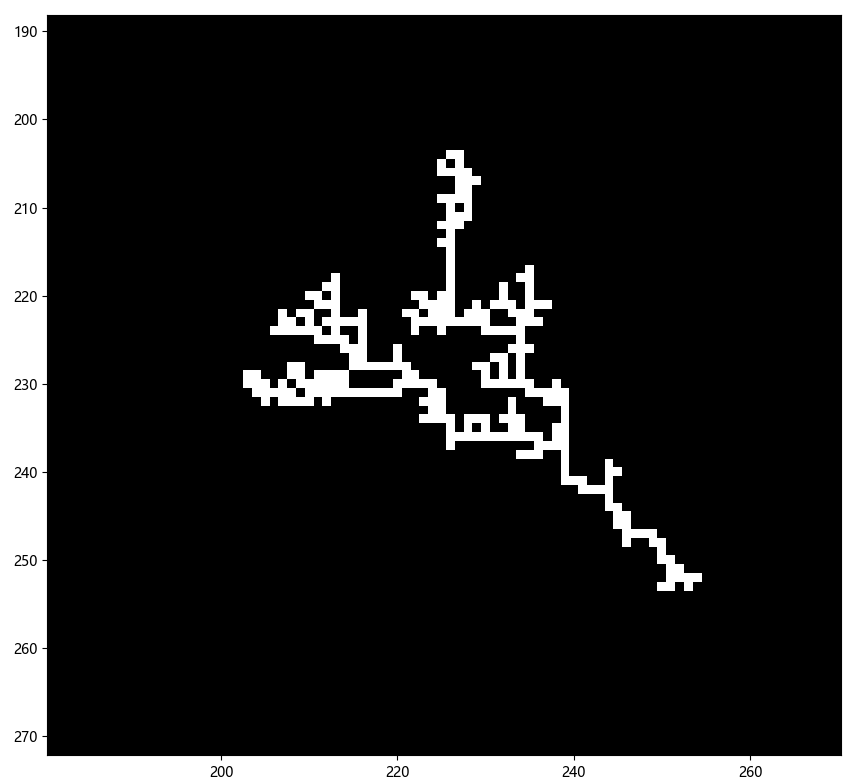
\includegraphics[scale=0.3]{DBM_3_300}}
	
	\subfigure[t=700]{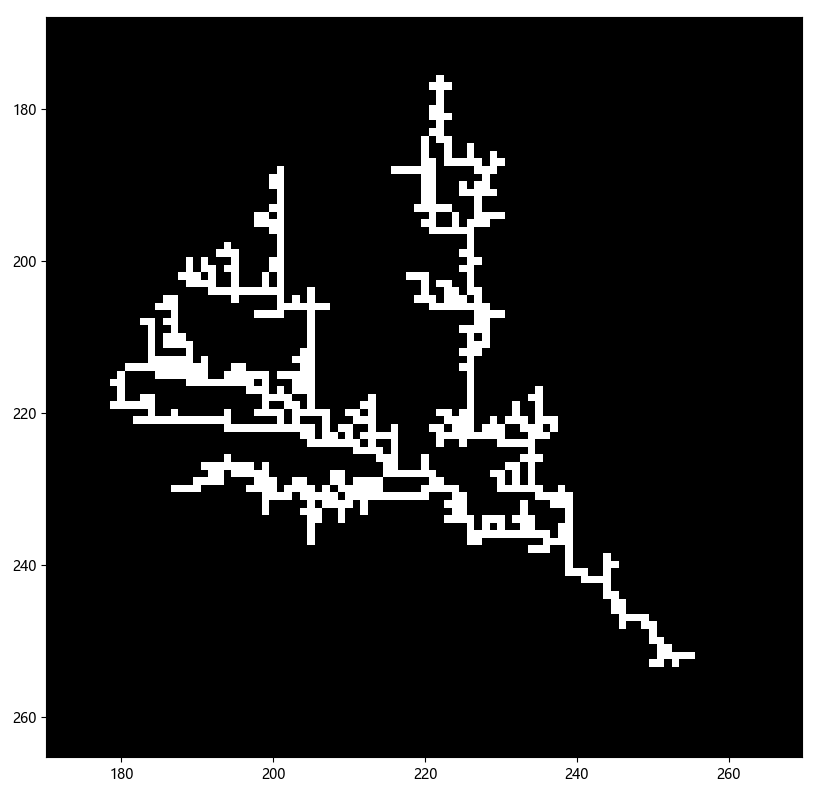
\includegraphics[scale=0.3]{DBM_3_700}}
	\subfigure[t=1000]{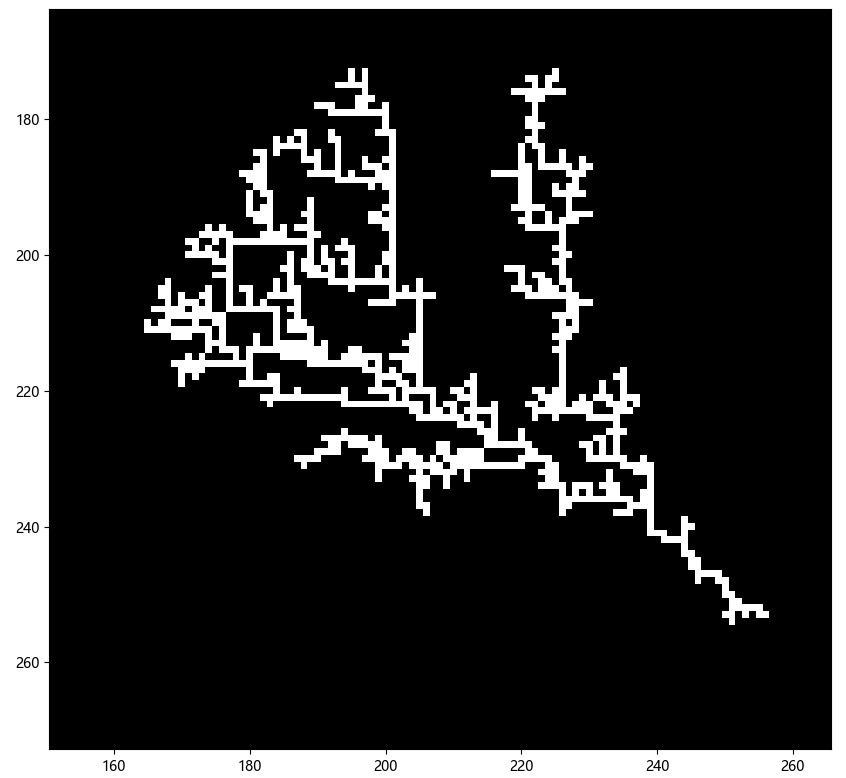
\includegraphics[scale=0.3]{DBM_3_1000}}
	\subfigure[t=1500]{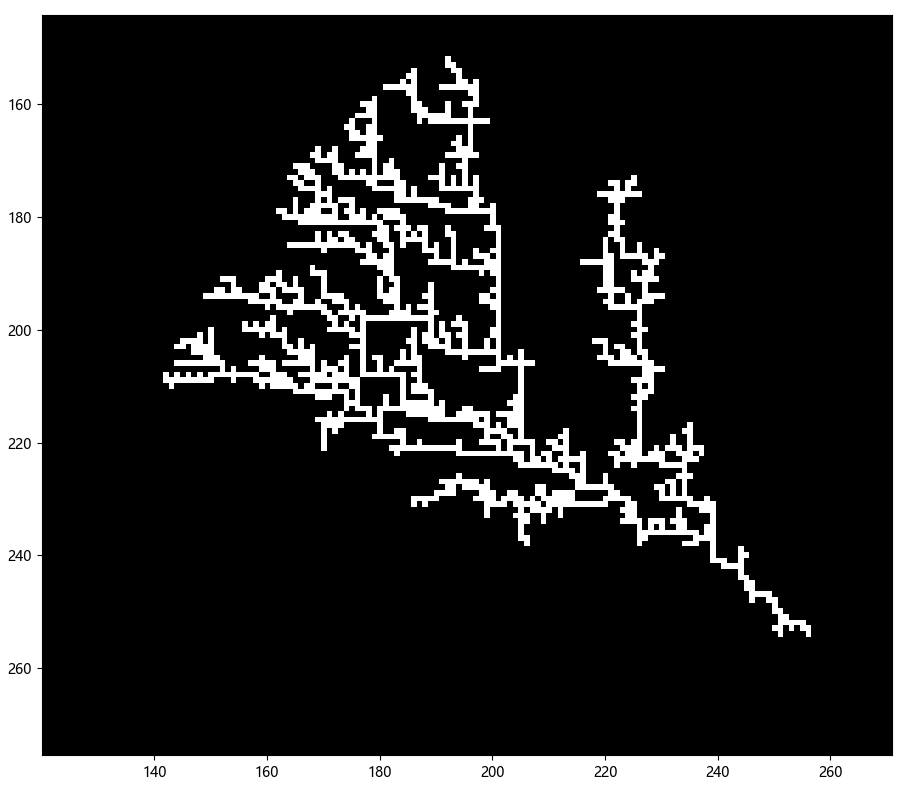
\includegraphics[scale=0.3]{DBM_3_1500}}
	\subfigure[t=2000]{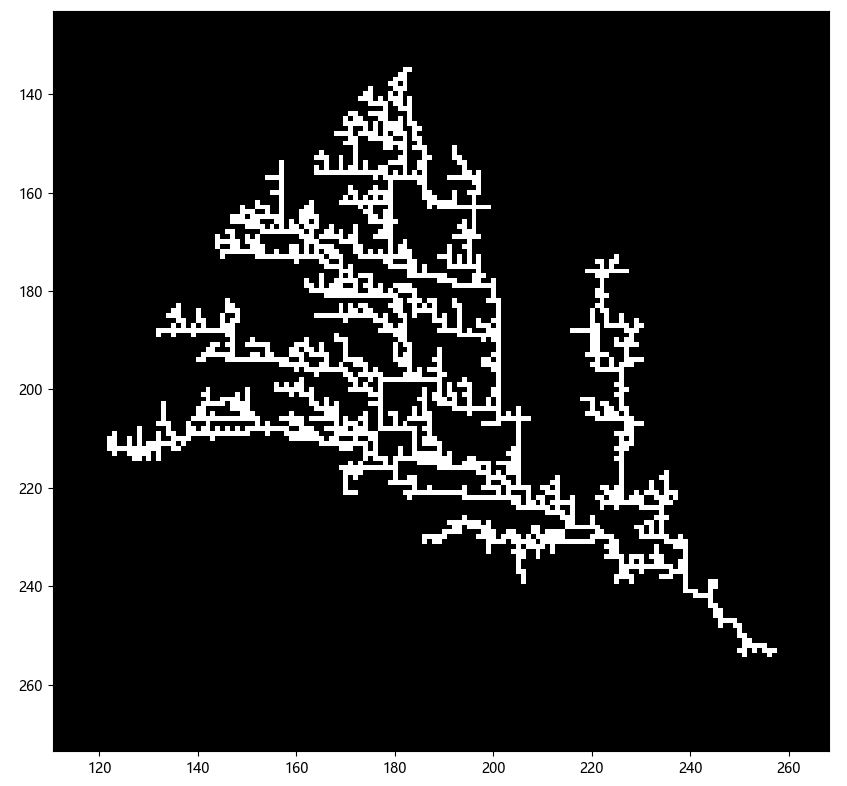
\includegraphics[scale=0.3]{DBM_3_2000}}
	\captionsetup{font={small},labelfont=bf}
	\caption{\heiti\zihao{-5}DBM生长($ \eta=3 $)}
	\label{fig:2}
\end{figure}


接下来图\ref{fig:3},\ref{fig:4},\ref{fig:5}分别计算了$ \eta=1,5,10 $下DBM生长情况。考虑到计算速度,取了生长次数t=100,300,700,1000
 \begin{figure}[!h]
	\centering
	\subfigure[t=100]{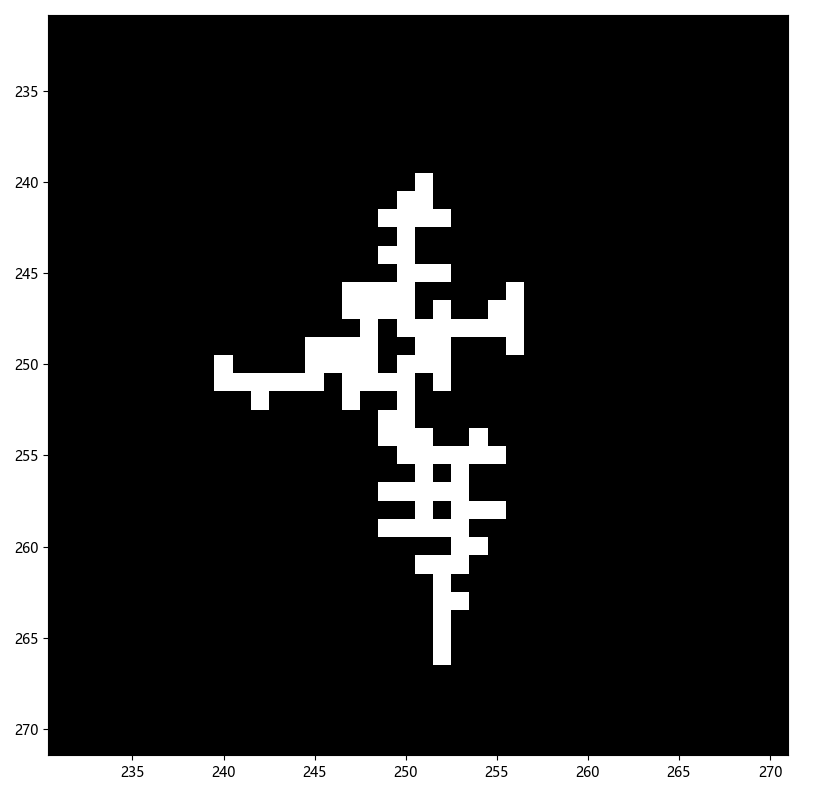
\includegraphics[scale=0.27]{DBM_1_100}}
	\subfigure[t=300]{	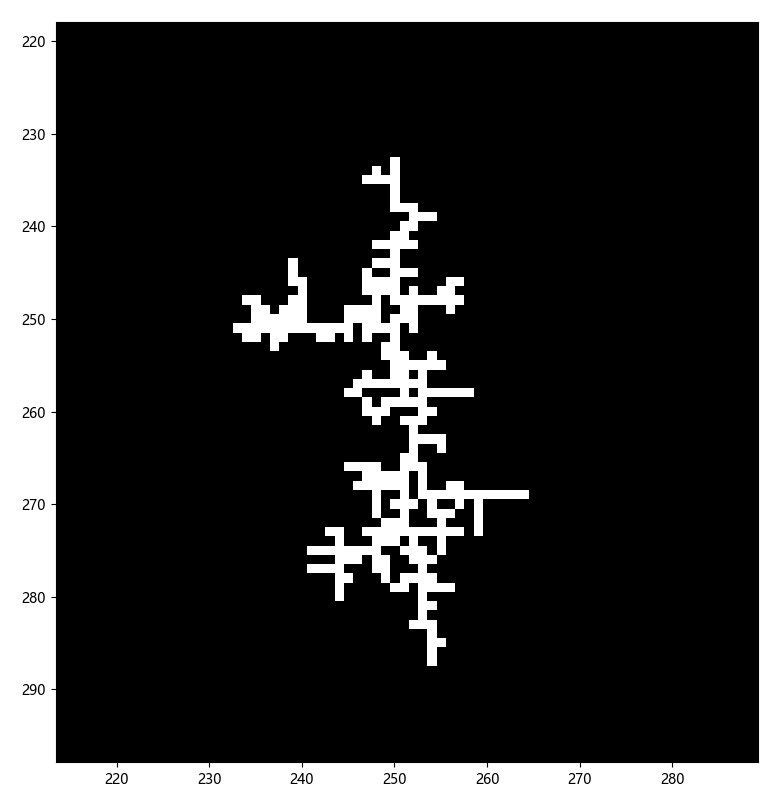
\includegraphics[scale=0.27]{DBM_1_300}}
	
	\subfigure[t=700]{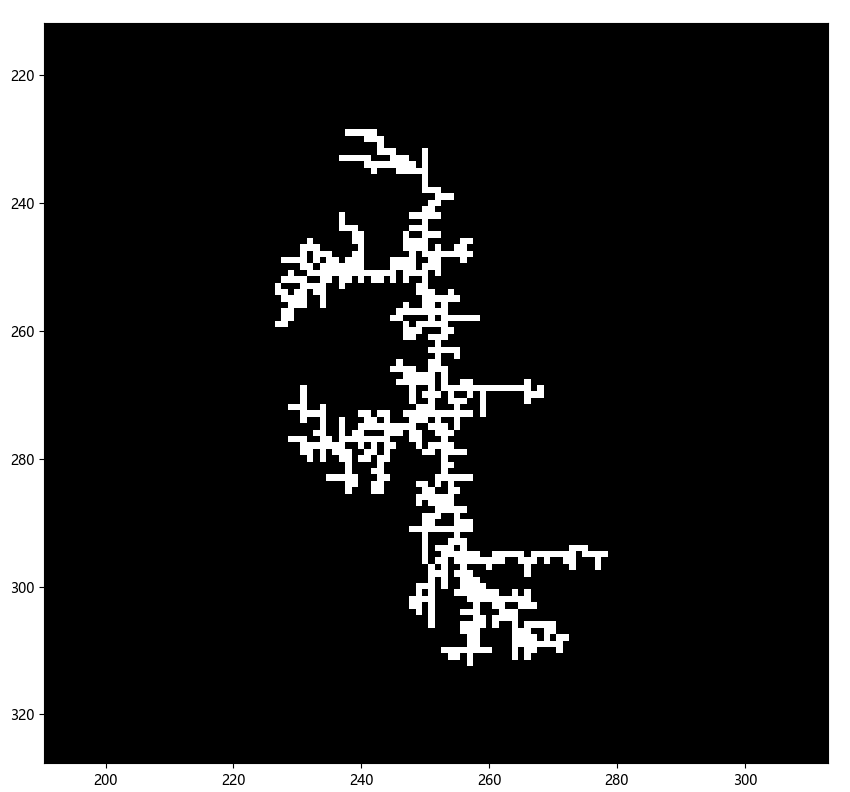
\includegraphics[scale=0.26]{DBM_1_700}}
	\subfigure[t=1000]{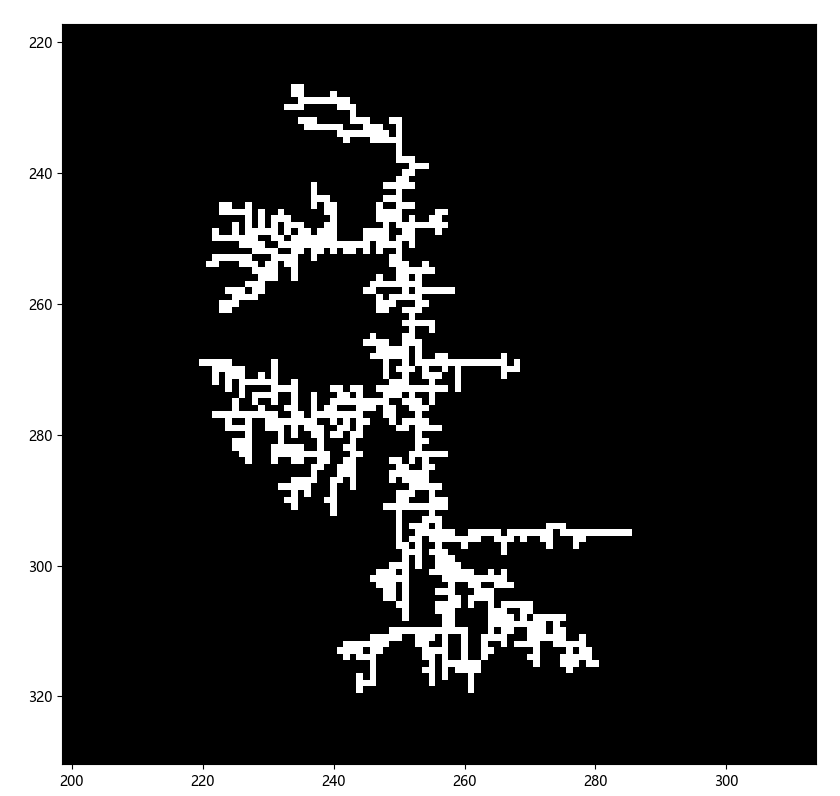
\includegraphics[scale=0.26]{DBM_1_1000}}
	\captionsetup{font={small},labelfont=bf}
	\caption{\heiti\zihao{-5}DBM生长($ \eta=1 $)}
	\label{fig:3}
\end{figure}
 \begin{figure}[!h]
	\centering
	\subfigure[t=100]{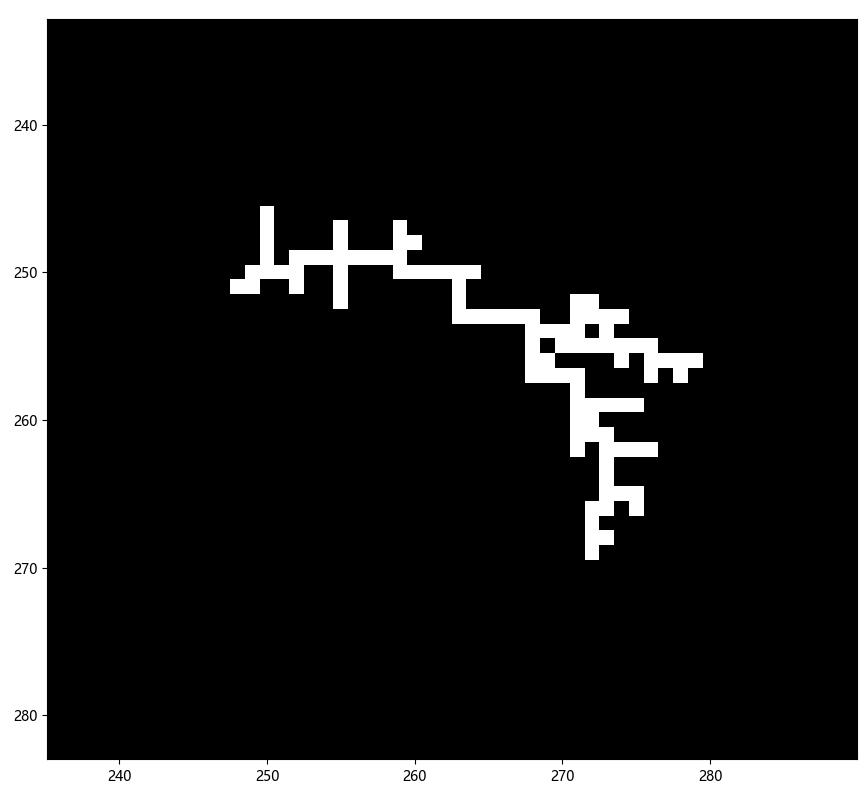
\includegraphics[scale=0.26]{DBM_5_100}}
	\subfigure[t=300]{	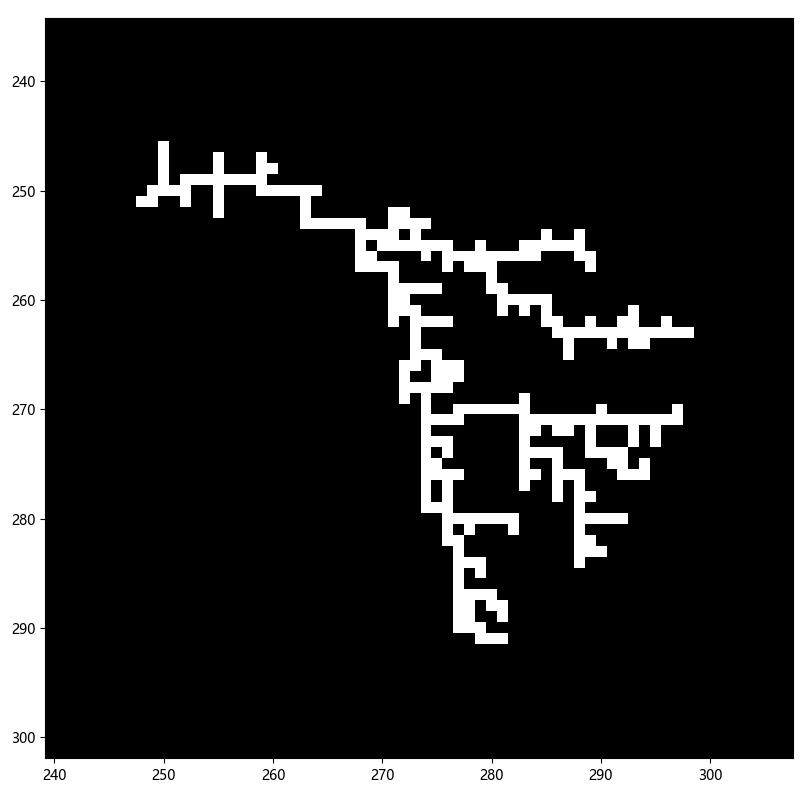
\includegraphics[scale=0.26]{DBM_5_300}}
	
	\subfigure[t=700]{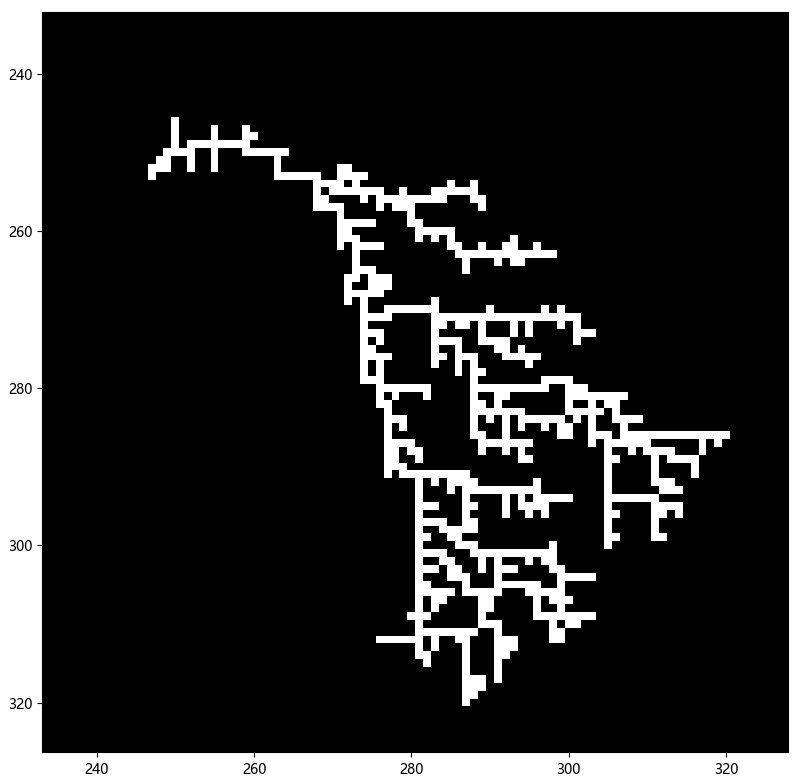
\includegraphics[scale=0.265]{DBM_5_700}}
	\subfigure[t=1000]{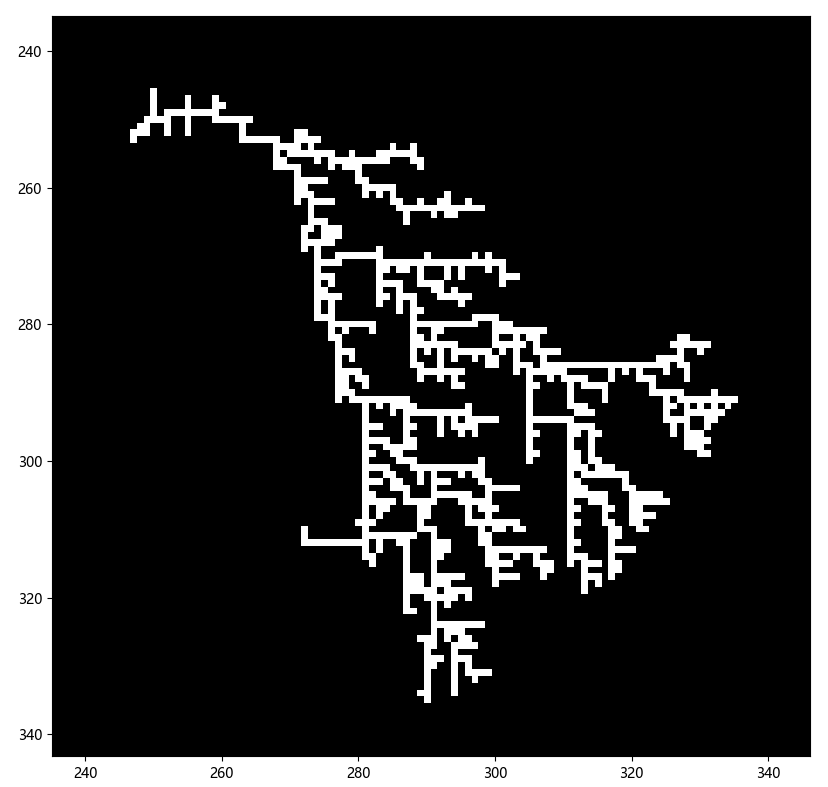
\includegraphics[scale=0.265]{DBM_5_1000}}
	\captionsetup{font={small},labelfont=bf}
	\caption{\heiti\zihao{-5}DBM生长($ \eta=5 $)}
	\label{fig:4}
\end{figure}
 \begin{figure}[!h]
	\centering
	\subfigure[t=100]{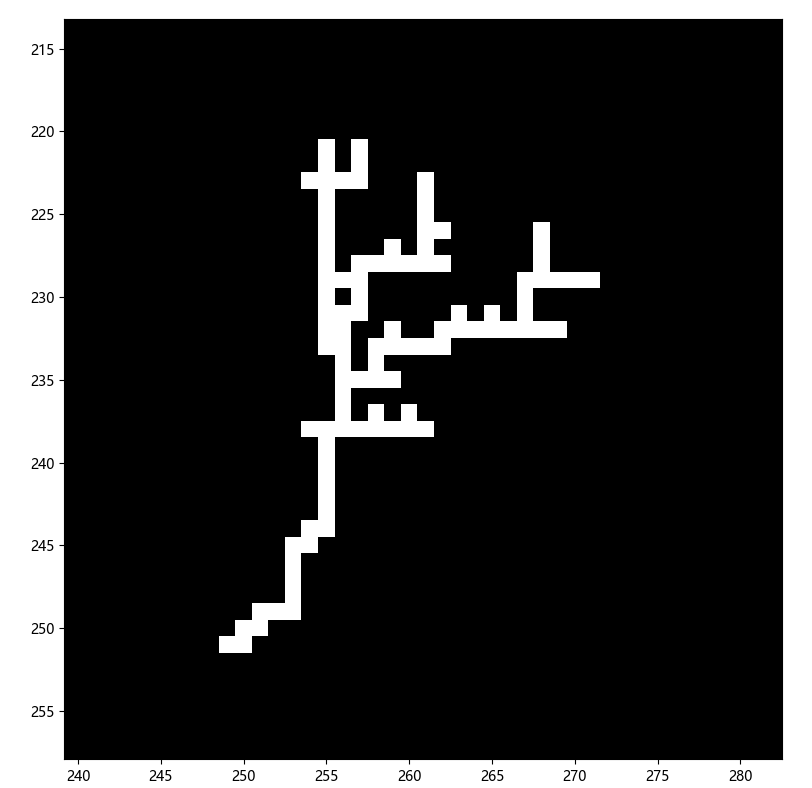
\includegraphics[scale=0.27]{DBM_10_100}}
	\subfigure[t=300]{	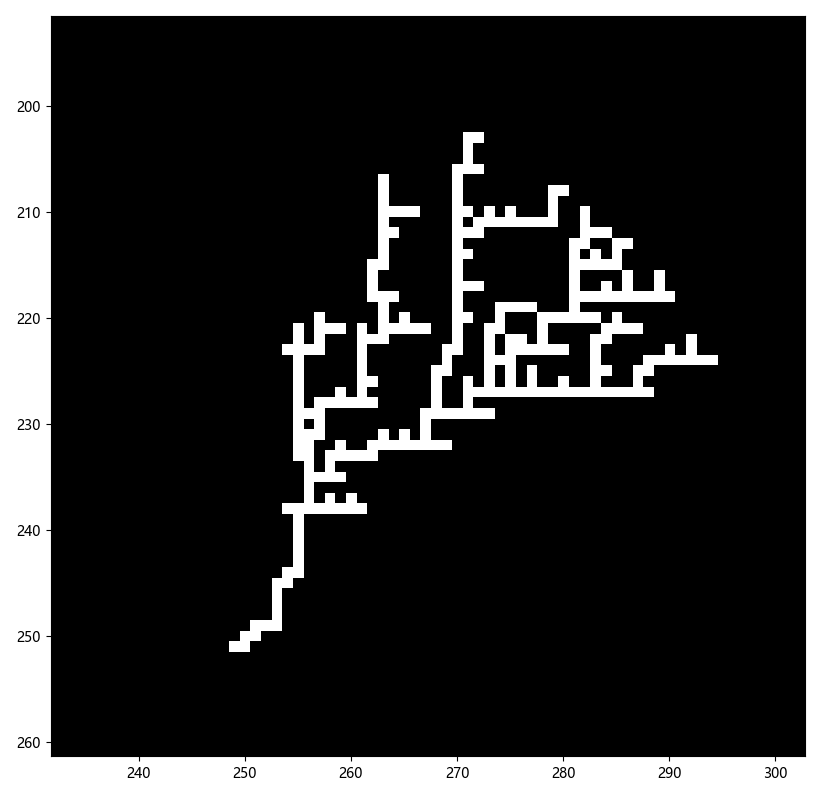
\includegraphics[scale=0.27]{DBM_10_300}}
	
	\subfigure[t=700]{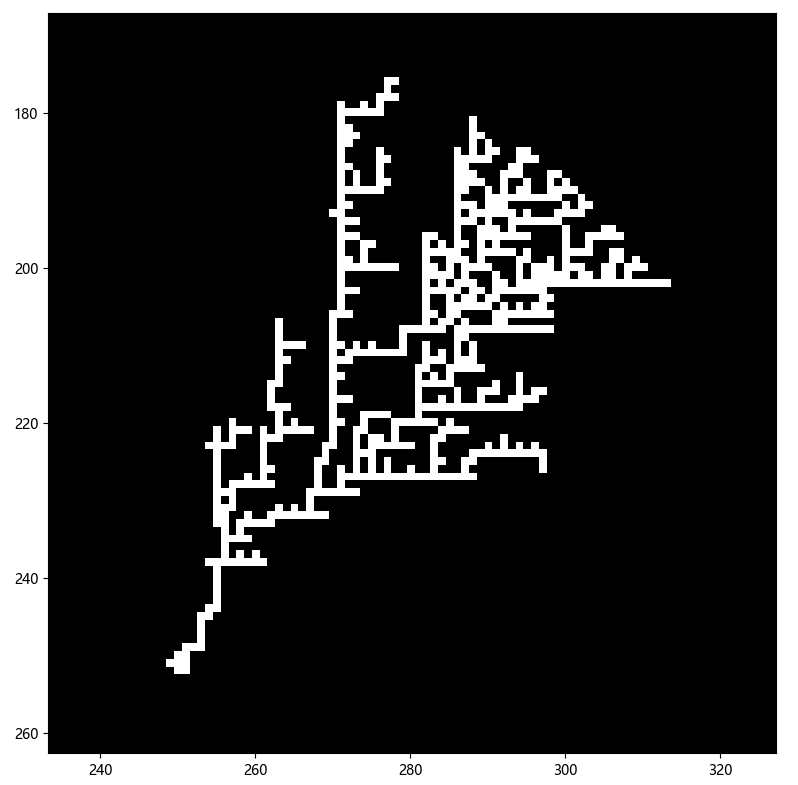
\includegraphics[scale=0.27]{DBM_10_700}}
	\subfigure[t=1000]{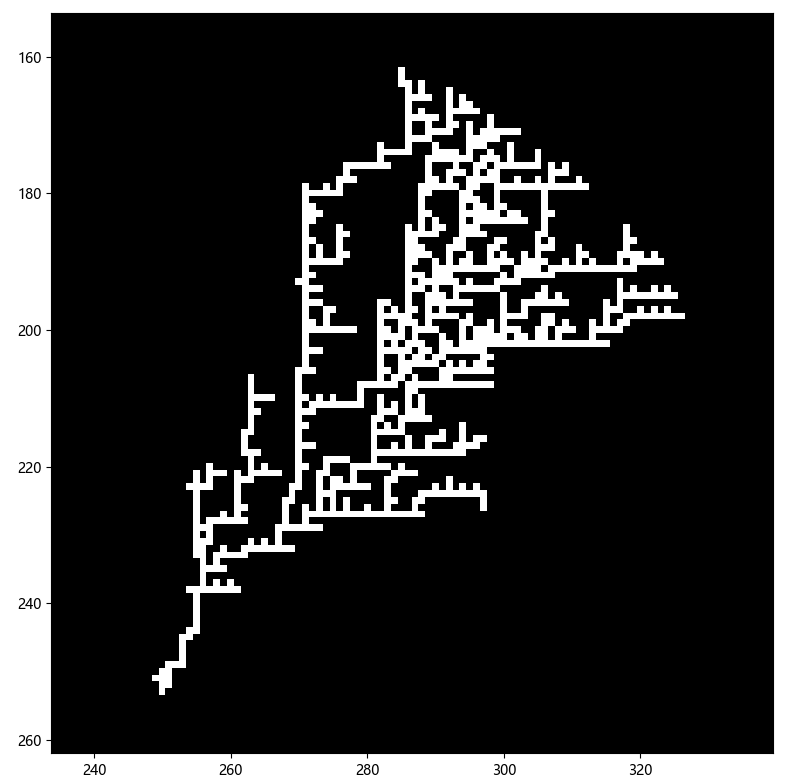
\includegraphics[scale=0.27]{DBM_10_1000}}
	\captionsetup{font={small},labelfont=bf}
	\caption{\heiti\zihao{-5}DBM生长($ \eta=10 $)}
	\label{fig:5}
\end{figure}
由图对比可见,当$ \eta $较小时,DBM生长接近于较为均匀的生长,而随着$  \eta $增大,DBM生长明显方向性增强,沿着尖端处生长趋势增强。对于该规律的解释为当$ \eta $作为电势梯度的幂次不断增大时,会导致电势梯度较大的点生长概率被放大,电势梯度小的点生长概率相对变小,导致沿尖端生长的趋势明显加强,生长的速度也会相应的加快。
	\section{结论}
本次实验模拟了DLA生长与DBM生长的图样,对比可得DBM生长明显具有更强的方向性,而DLA生长则相对更加均匀的在网格上铺开。同时由于DBM生长具有偏压特性,其生长速率较DLA更快,在相同时间内生长延伸的较远。而且DBM生长方向明显具有较强的随机性,主要取决于初始时刻生长的方向,会导致之后整体生长的方向会不稳定地倒向初始生长方向。相比之下DLA生长的均匀性较为稳定。
\end{document}